\section{La fase de entrenamiento}
\label{sec:EntrenamientoPython}

En este apartado se describen las fases de entrenamiento de los modelos, así como la evolución de los mismos y la serie de decisiones tomadas para conseguir esas adaptaciones. El código al que se hace referencia puede encontrarse en el directorio /Entrenamiento del repositorio de GitHub del proyecto \footnote{Enlace a la carpeta de entrenamiento: \url{https://github.com/mikeletzu/TFG_FisicaOptim/tree/23105b6733cacae9c708593f2d77a12faa2eb884/Entrenamiento}}. 

\subsection{El entorno de trabajo}

Para crear un entorno de trabajo adaptable, y asegurar la consistencia entre los distintos equipos utilizados por las integrantes de este proyecto, se ha decidido crear en el repositorio un archivo \textit{dl2024\_gpu.yml} en el que concretar las dependencias del proyecto y las versiones a utilizar de estas librerías. Este es un tipo de archivo de configuración que permite, entre otras cosas, crear fácilmente Conda Environments. Estos entornos virtuales se generan en un directorio con todas las dependencias especificadas. Se ha utilizado como base el entorno propocionado por la Universidad de Amsterdam en sus cursos introductorios de Deep Learning con Pytorch.
\begin{table}[H]
    \begin{center}
        \begin{tabular}{ | m{4cm} | m{2cm} | }
        \hline Librerias utilizadas & Versiones \\ \hline
            python & 3.12.7 \\ \hline
            cmake & - \\ \hline
            notebook & 7.2.2 \\ \hline 
            jupyterlab & 4.2.5 \\ \hline 
            matplotlib & 3.9.2 \\ \hline 
            scikit-learn & - \\ \hline
            pytorch-cuda & 11.8 \\ \hline
            pytorch & 2.5.0 \\ \hline
            onnx & 1.21.0 \\ \hline
            onnxruntime & 1.24.2 \\ \hline
            onnxscript & 0.5.6 \\ \hline
            skl2onnx & 1.20.0 \\ \hline
        \end{tabular}
    \end{center}
    \caption{Librerías y versiones del entorno de desarrollo.}
\end{table}

\subsection{Apartados de la ejecución del entrenamiento}

Dada su flexibilidad para segmentar la ejecución y su capacidad de visualizar los resultados claramente, se ha elegido IPython Notebook (.ipynb) como como herramienta de desarrollo en python. Si bien cada tipo de modelo se ha creado en un archivo distinto, todos comparten la misma estructura. Pese a la inevitable repetición de código y potencial optimización, la utilización de diferentes notebooks ha resultado clave para el desarollo e investigación paralela de los diferentes modelos. La estructura tiene la siguiente forma: ESTO HAY QUE CAMBIARLO tt

\begin{enumerate}

    \item \textbf{Carga y procesamiento de datos}: 
    Los datos se leen del archivo .csv utilizando la librería pandas, que permite llevar a cabo la limpieza fácilmente. Aunque es el dataset del modelo quien gestiona detalles como la coherencia de frames otorgados, intentar acceder al predecesor de un primer frame, se realiza una limpieza común previa del csv:
    \begin{itemize}
        \item Se elimina la columna "frame"\ de la tabla, ya que no aporta información pertinente para el aprendizaje. Su función es meramente auxiliar para depurar.
        \item Asímismo, en los casos que se explicarán más adelante, muchos de los parámetros registrados no son necesarios, se filtran esas columnas para no sobrecargar innecesariamente el dataset.
    \end{itemize}
    Tras hacer la limpieza de los datos estos se transforman al formato de tensores de Pytorch. 

    \item \textbf{Dataset de Pytorch}: Pytorch ofrece dos clases base con las que ordenar y gestionar los datos que requiere el modelo. \textit{Torch.utils.data.Dataset} almacena las muestras y sus etiquetas correspondientes, y \textit{torch.utils.data.DataLoader} permite un fácil acceso a las muestras. En este bloque se definen las carácteristicas del Dataset en base a las necesidades del modelo; este recibe en su constructora el tensor con la información filtrada y el tamaño de los lotes en los que dividirlo.

    \item \textbf{Normalización}: Se dividen los datos siguiendo un split temporal, donde el primer 80\% de los frames se utilizan para el entrenamiento y el 20\% respante para las pruebas. Se itera sobre los datos de entrenamiento para calcular los deltas\footnote{\textbf{Deltas:} Hace referencia al desplazamiento de cada vértice en cada frame en los ejes X, Y y Z.} y se normaliza tanto el input completo como los deltas generados para los datos de entrenamiento. La normal y la desviación típica tanto del input como del target se guardan el un archivo de formato JSON \textit{cloth\_norm\_params.json}. Posteriormente, estos datos se utitizan para generar el input del modelo en la ejecución de Unity, ya que este requiere que la estandarización de los datos con los que se entrenó la red sea la misma que la de los datos en ejecución.

    \item \textbf{Modelo de Pytorch}: Pytorch ofrece también una clase base a partir de la cual implementar modelos de redes neuronales, \textit{torch.nn.Module}. En este apartado se extiende esta clase a las especificaciones deseadas y se genera utilizando el DataLoader mencionado un primer batch de prueba.
    
    \item \textbf{Entrenamiento}: En este apartado se determinan los parámetros del entrenamiento: \textit{learning rate}, iteraciones, porcentaje de ruido y etc. El entrenamiento consiste en una fase de entrenamiento y otra de testing, en la que se observa el aprendizaje del modelo através de la caída del error medio de la posición de cada vértice.
    
    \item \textbf{Visualización de resultados}: Al trabajar con una simulación físca en un entorno 3D, la visualización en gráficos de las predicciones de los modelos ha resultado notablemente útil. En las figuras \ref{fig:visualA}, \ref{fig:visualB} y \ref{fig:visualC} pueden apreciarse los gráficos más destacados que más han contribuido al desarollo.        
        \begin{figure}[H]
            \centering
            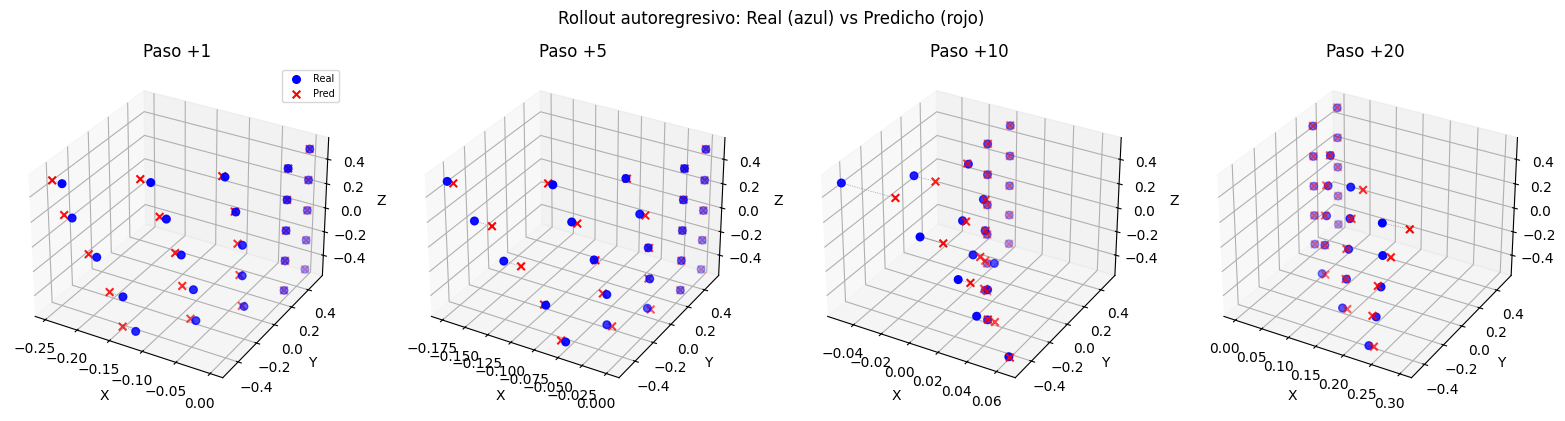
\includegraphics[width=0.91\textwidth]{Imagenes/ejemploVisualA.png}
            \caption{Visualización de los puntos de la tela simulada e inferida a lo largo del tiempo.}
            \label{fig:visualA}
        \end{figure}
        \begin{figure}[H]
            \begin{minipage}{0.48\textwidth}
                \centering
                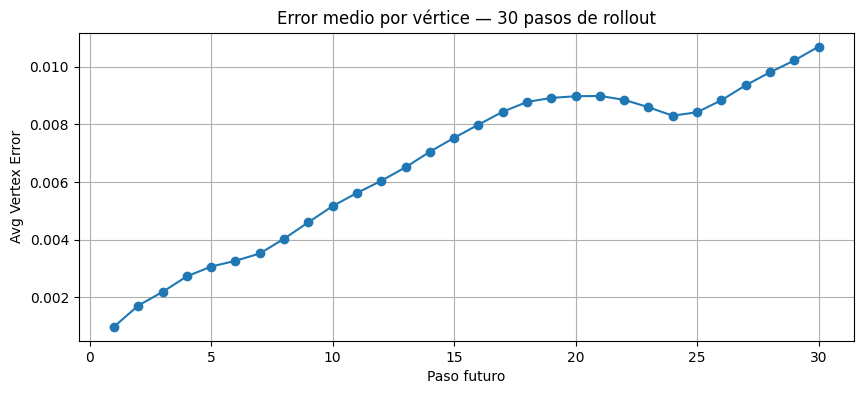
\includegraphics[width=\textwidth]{Imagenes/ejemploVisualB.png}
                \caption{Visualización del error medio a lo largo del tiempo}
                \label{fig:visualB}
            \end{minipage}
            \hfill
            \begin{minipage}{0.48\textwidth}
                \centering
                
\includegraphics[width=\textwidth]{Imagenes/ejemploVisualC.png}
                \caption{Visualización de error de normalización}
                \label{fig:visualC}
            \end{minipage}
        \end{figure}
    
    \item \textbf{Exportación}: Por último, tras considerar los resultados generados como adecuados con la guía de los valores y gráficas generadas, se procede a exportar la red neuronal a formato ONNX.
\end{enumerate}

\subsection{Modelos}
Los modelos entrenados infieren la diferencia de desplazamiento entre un frame y el siguiente. Utilizan como función de pérdida \textit{L1Loss}\footnote{\textbf{L1Loss:} Función proporcionada por Pytorch que calcula el error absoluto medio entre los valores predichos y los valores reales.} de la posición y la velocidad. El input se construye con el SDF, la posición y velocidad de los vértices normalizados con inyección de ruido aolanados en un vector y como output se obtienen los deltas de desplazamiento normalizados. Estos deltas de posición se añaden a las posiciones del frame actual para obtener el siguiente paso de la simulación. \newline

Como se ha mencionado previamente, hay dos nociones principales que han guiado el desarrollo de este proyecto. Por un lado, combinar las técnicas óptimas o prometedoras de las investigaciones citadas en el estado del arte. Y por otro, priorizar la simplicidad y accesibilidad de nuestro modelo en la plataforma elegida. Hemos seleccionado redes específicas y características que han permitido llegar a un movimiento de una tela coherente. Estas son las siguientes características que conforman nuestros modelos, y sobre las cuales se harán comparativas en el apartado de experimentos.

\subsubsection{Gestión de error acumulado}
\begin{figure}[H]
        \centering
        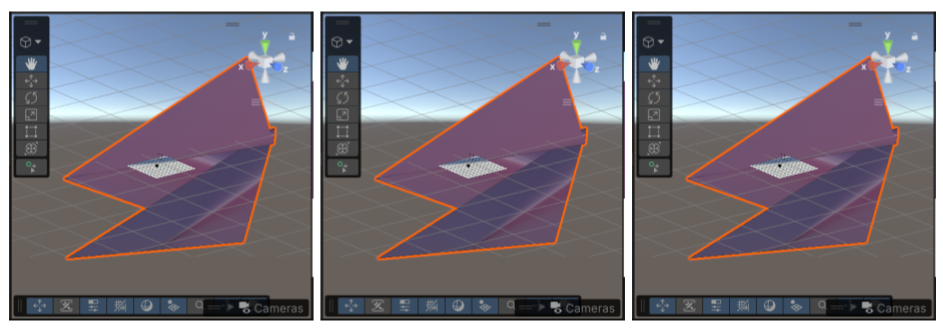
\includegraphics[width=0.91\textwidth]{Imagenes/errorAcumulado.png}
        \caption{Error acumulado}
    \end{figure}

En primer lugar, se incorporan diferentes técnicas que ayudan a estabilizar el error acumulado de distancia de vértices. Estas permiten que el aprendizaje pueda aprender a autocorregirse y conservar la geometría original de la tela, así como evitar movimientos extremos a medida que avanza la simulación. Son las siguientes:
\begin{itemize}
    \item \textbf{Ruido en el input:} Una de las técnicas más sencillas para mejorar la capacidad del modelo de corregir sus errores es entrenarlo creando pequeños errores de forma artifical. Esto se consigue añadiéndole ruido a los datos de entrada, en este caso se añade un ruido gaussiano de entre un 2 y un 5\% de magnitud respecto a los datos de entrada antes de normalizar. De esta manera, el modelo aprende a corregir estos errores para corregir los suyos propios en un futuro.
    
    \item \textbf{Unrolling for training:} La idea de dividir el entrenamiento en distintos modelos es habitual; ya sea con una red que dé resultados más generales y una segunda que consiga refinar los detalles (arrugas, intersecciones con el colisionador, etc.) como en TailorNet \cite{patel2020tailornet}, o con modelos que actúen como predictor-corrector siendo el segundo normalmente en post-procesado. Sin embargo, en este proyecto se propone incluir esta idea en el propio entrenamiendo del modelo, con la función de pérdida. El caso de \cite{chen2025learning}, por ejemplo, el concepto de una función de pérdida \textit{force-inpulse} que penaliza tanto el error en la fuerza predicha como el inpulso que esta genera para las siguientes inferencias. De manera similar, en este proyecto se genera una secuencia de predicciones; la cadena de deltas generados sucesivamente permiten al modelo tener una noción sobre el cambio de velocidad y aceleración provocados. 
    
    La implementación que se incorpora en este proyecto se inspira más en la investigación de \cite{holden_subspace_2019}, en la que se lleva acabo un proceso similar. Además de retroalimentar los frames generados a la secuencia de input, se propaga el error utilizando la técnica BPTT (\textit{Backpropagation Through Time}). Esta técnica consiste en retropropagar el error a lo largo de la secuencia temporal y permite a la red aprender dependencias temporales.
    
    \begin{itemize}
        \item \textbf{Ventana inicial:} $V_0 = [y_{t-n+1}, \dots, y_t]$
        \item \textbf{Bucle de predicción:} Para $i = 1, 2, \dots, W$:
        \begin{enumerate}
            \item Calcular predicción: $\hat{y}_{t+i} = f(V_{i-1})$
            \item Actualizar ventana: $V_i = [V_{i-1} \setminus \{y_{primero}\}] \cup \{\hat{y}_{t+i}\}$
        \end{enumerate}
        \item \textbf{Función de pérdida (Loss):} 
        $$\mathcal{L} = \frac{1}{W} \sum_{i=1}^{W} (y_{t+i} - \hat{y}_{t+i})^2$$
    \end{itemize}
\end{itemize}

\subsubsection{Tipos de redes y recurrencia}
En este estudio nos hemos enfocado en dos tipos de redes neuronales que se alienan con nuestro objetivos de emplear modelos sencillos: los \textbf{perceptrones multicapa (MLP)} y las \textbf{redes neuronales recurrentes (RNN)}. Otras redes como las CNN o las GNNS han sido descartados debido a la alta complejidad para representar y proporcionar los datos al modelo.

\begin{itemize}
    \item \cite{holden_subspace_2019} resalta el MLP como una red sencilla computancionalmente más accesible que las CNNs empleadas en otros estudios, manteniendo la capacidad de proporcionar resultados adecuados mediante su uso de subespacios y correcciones. 
    \item Por otra parte, empleamos una RNN para comprobar si la memoria recurrente ayuda a gestionar mejor el movimiento dinámico y conservar la geometría a través del tiempo. Varias de las investigaciones del estado del arte, como por ejemplo \cite{santesteban2022snug}, mencionan como limitación las telas más dinámicas, ya que, al tener muchas menos restricciones, las mallas que no van pegadas a un cuerpo de colisión son mucho más susceptibles a la inercia. Naturalmente, el aprendizaje de estas propiedades físicas requiere del conocimiento de atributos como la velocidad o la aceleración de las partículas. La recurrencia permite al modelo tener una memoria a corto plazo del movimiento en cada vértice, haciendo su entrenamiento mucho más eficaz. Sigue la arquitectura de tipo "many to one", donde una cantidad determinada de frames se utilizan como input para generar el delta de desplazamiento entre el último frame de la secuencia y el que sería el siguiente.
\end{itemize}



\subsubsection{Reducción de dimensionalidad}
Para conseguir alcanzar una mejora de rendimiento y complejidad en los modelos, se necesita reducir la dimensionalidad de las entradas y salidas del modelo. Encontramos distintas formas de reducir, como 
El PCA se usa ampliamente para conservar las deformaciones principales en simulaciones complejas, pudiendo compactar la informacion y reducir la complejidad. Se pasa al modelo unos coeficientes del subespacio PCA y se reconstruye de vuelta en Unity! :3

Aplicamos un PCA con un número de componentes que respeta que el umbral de varianza esté sobre el 95\%. En el caso de este estudio, X componentes.

\begin{figure}[H]
    \centering
        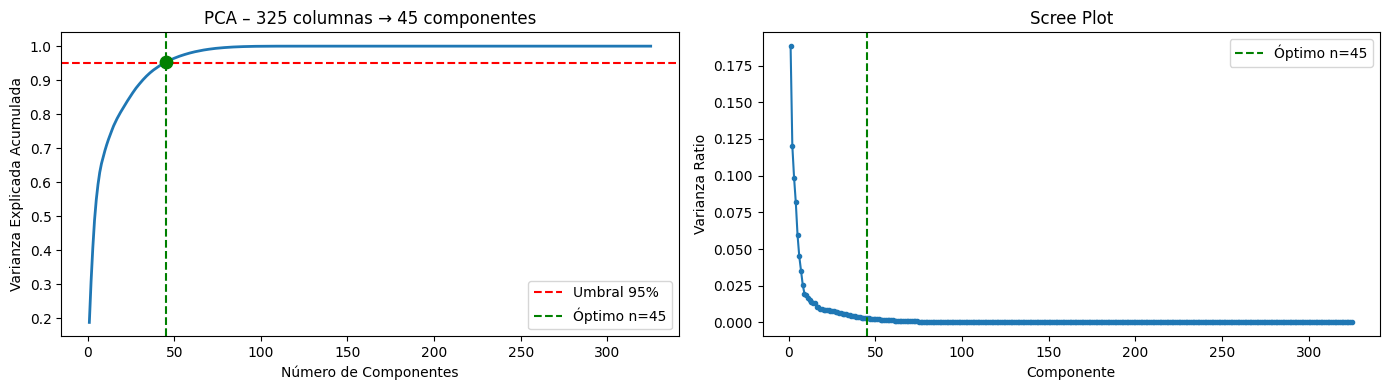
\includegraphics[width=0.91\textwidth]{Imagenes/resultPCA.png}
        \caption{Componentes óptimas para PCA}
\end{figure}

Se calculan los frames con el PCA aplicados necesarios para realizar todas las predicciones de
\subsection{Resultado e hiperparámetros}

Tras el proceso de iteraciones descrito, se concluye que la red neuronal más óptima es una RNN con \textit{unrolling}, utilizando como función de pérdida \textit{L1Loss}\footnote{\textbf{L1Loss:} Función proporcionada por Pytorch que calcula el error absoluto medio entre los valores predichos y los valores reales.} de la posición y la velocidad. El input se construye con el SDF, la posición y velocidad de los vértices normalizados con inyección de ruido y como output se obtienen los deltas de desplazamiento normalizados.\newline
La siguiente función, \textit{RunRollout()}, lleva a cabo el cálculo de las predicciones y la pérdida de las mismas para cada lote de datos del dataset. Siguiendo la técnica mencionada, ejecuta las predicciones necesarias para avanzar en el tiempo tanto como el tamaño de la ventana de unrolling le indica. Por simplicidad el modelo que sa ha decidido representar por pseudocódigo recoge únicamente la posición y sdf como parámetro de entrada.

\begin{comment}
\begin{algorithm}[H]
\caption{Función de \textit{Unrolling}}
\label{alg:run_rollout}
\begin{algorithmic}[1]
\Function{RunRollout}{$ batch\_seq, batch\_future$}
    \State $B, W, V, F \gets \text{dimensiones de } batch\_future$
    \State $window \gets \text{copia}(batch\_seq)$ \Comment{La copia permite no alterar el tensor original}
    %\BlankLine
    \State \textbf{\textit{Inyección de ruido inicial}}
    \State $noise \gets \mathcal{N}(0, \sigma_{\text{noise}}) \text{ del mismo tamaño que } window[:, -N:]$
    \State $window[:, -N:] \gets window[:, -N:] + noise$
    
    %\BlankLine
    \State \textbf{\textit{Iteración sobre la secuencia}}
    \State $total\_loss \gets 0$
    \State $prev\_pred\_pos \gets window[:, -1, :, 0:3]$ \Comment{Posición en $t-1$}
        
    %\BlankLine
    \For{$k \gets 0$ \textbf{to} $W - 1$}
        \State $window\_norm \gets \text{NormalizarEntrada}(window)$
        \State $ pred\_delta\_norm \gets \text{Modelo}(window\_norm)$ \Comment{Inferencia de la red}        
        \State $ last\_pos \gets window[:, -1, :, 0:3]$
        \State $ pred\_delta\_real \gets \text{DesnormalizarDelta}(pred\_delta\_norm)$
        \State $ pred\_pos \gets last\_pos + pred\_delta\_real$ \Comment{Nueva posición absoluta}
        
        %\BlankLine
        \State $real\_pos \gets batch\_future[:, k, :, 0:3]$
        \State $real\_prev\_pos \gets (k > 0) \mathrel{?} batch\_future[:, k-1, :, 0:3] : batch\_seq[:, -1, :, 0:3]$
        
        %\BlankLine
        \State $real\_delta\_norm \gets \text{NormalizarDelta}(real\_pos - last\_pos)$
        \State $loss\_pos \gets \mathcal{L}_{L1}(pred\_delta\_norm, real\_delta\_norm)$ \Comment{Cálculo del Loss de Posición}
        
        %\BlankLine
        \State $pred\_vel \gets pred\_pos - prev\_pred\_pos$
        \State $real\_vel \gets real\_pos - real\_prev\_pos$
        \State $loss\_vel \gets \mathcal{L}_{L1}(pred\_vel / \sigma_{target}, real\_vel / \sigma_{target})$ \Comment{Cálculo del Loss de Velocidad}
        
        %\BlankLine
        \State $total\_loss \gets total\_loss + loss\_pos + (\gamma_{vel} \times loss\_vel)$
        
        %\BlankLine
        \Comment{\textit{Feedback Loop}}
        \State $new\_frame \gets \text{ConstruirFrame}(pred\_pos, \text{resto de propiedades reales})$
        \State $window \gets [window[:, 1:], new\_frame]$ \Comment{Desplazar ventana temporal}
        \State $prev\_pred\_pos \gets pred\_pos$
    \EndFor 
    \State \Return $total\_loss / W$
\EndFunction
\end{algorithmic}
\end{algorithm}
\end{comment}
La siguiente sección de pseudocódigo describe el bucle para llevar a cabo el entrenamiento completo del modelo. Inicialmente, se dividen los datos de entrenamiento en lotes, estos contienen una secuencia de entrada para el modelo y la secuencia de frames inmediatamente posterior. Con estos datos y la función descrita anteriormente, se obtiene la pérdida del modelo para la retropropagación y se actualizan sus pesos. La fase de evaluación también utiliza la función anterior para analizar la calidad del modelo ante situaciones nuevas, y calcula el primer frame de cada lote para obtener una aproximación de la media de error en la predicción de los deltas.

\begin{comment}
\begin{algorithm}[H]
\caption{Bucle de Entrenamiento y Validación}
\label{alg:training_loop}
\begin{algorithmic}[1]
\For{$epoch \gets 1$ \textbf{to} $\text{EPOCHS}$}
    
    \State\textbf{Fase de Entrenamiento (Train)}
    \State Establecer modelo en modo entrenamiento
    \State $train\_loss \gets 0.0$
    \For{cada $(batch\_seq, batch\_future)$ en $train\_loader$}
        \State $loss \gets \textsc{RunRollout}(batch\_seq, batch\_future)$
        \State $\text{Optimizador.zero\_grad}()$
        \State $loss.\text{backward}()$
        \State $\text{RecortarGradientes}(model.parameters, \text{umbral}=1.0)$
        \State $\text{Optimizador.step}()$
        \State $train\_loss \gets train\_loss + loss.\text{item}()$
    \EndFor

    \State $\text{Planificador.step}()$ \Comment{Actualizar tasa de aprendizaje}
    
    \State\textbf{Fase de Evaluación (Test)}
    \State Establecer modelo en modo evaluación y desactivar gradientes
    \State $test\_loss \gets 0.0$, $total\_err \gets 0.0$, $total\_verts \gets 0$

    \For{cada $(batch\_seq, batch\_future)$ en $test\_loader$}
        \State $loss \gets \textsc{RunRollout}(batch\_seq, batch\_future)$
        \State $test\_loss \gets test\_loss + loss.\text{item}()$
        
        \Comment{Métricas de error en el primer paso ($k=0$)}
        \State $pred\_pos \gets \text{PredecirSiguientePaso}(batch\_seq)$
        \State $target\_pos \gets batch\_future[:, 0, :, 0:3]$
        \State $distancias \gets \|pred\_pos - target\_pos\|_2$
        \State $total\_err \gets total\_err + \sum(distancias)$
        \State $total\_verts \gets total\_verts + \text{NúmeroDeElementos}(distancias)$
    \EndFor
    \State $\text{ErrorVértice} \gets total\_err  /  total\_verts$
    \State Almacenar métricas medias del $epoch$ en el historial
    \State Imprimir en consola: $epoch$, $train\_loss$, $test\_loss$, $\text{ErrorVértice}$
\EndFor
\end{algorithmic}
\end{algorithm}

\end{comment}
Para acabar de ajustar el modelo se itera sobre los mismos datasets modificando los parámetros variables.
\begin{itemize}
    \item \textbf{Windows size:} Cantidad de frames de la secuencia de input, esta actuará como ventana deslizante conforme se añadan los frames predichos.
    \item \textbf{Rollout steps:} Cantidad de frames que el modelo produce en el unroll.
    \item \textbf{Noise:} Se varía en la cantidad proporcional de ruido en el input normalizado (entre un 2 y un 5 \%) y este se aplica a los últimos n frames de la ventana del input.
    \item \textbf{Learning rate:} Se reduce la tasa de aprendizaje cuando este se estanca.
    \item \textbf{Tamaño dataset:} Se varía entre datasets desde 5000 a 25000 frames para determinar el tamaño mínimo con el que se consigue un resultado apropiado.
    \item \textbf{Batch size:} Este depende del tamaño del dataset y el detalle que se esté dispuesto a sacrificar para reducir el tiempo de entrenamiento.
\end{itemize}